% !TEX root = ../../I4PRJ, Grp3 - Dokumentation.tex
\chapter{Arkitektur}
I dette afsnit beskrives den overordnede arkitektur for systemet. Systemets arkitektur har dannet ramme for design og senere implementering. Domæneanalyse giver anledning til en 3-tier arkitektur, da systemet har tre domæner, som er application, server og database.

\section{3 Tier Model}
\begin{figure}
	\centering
	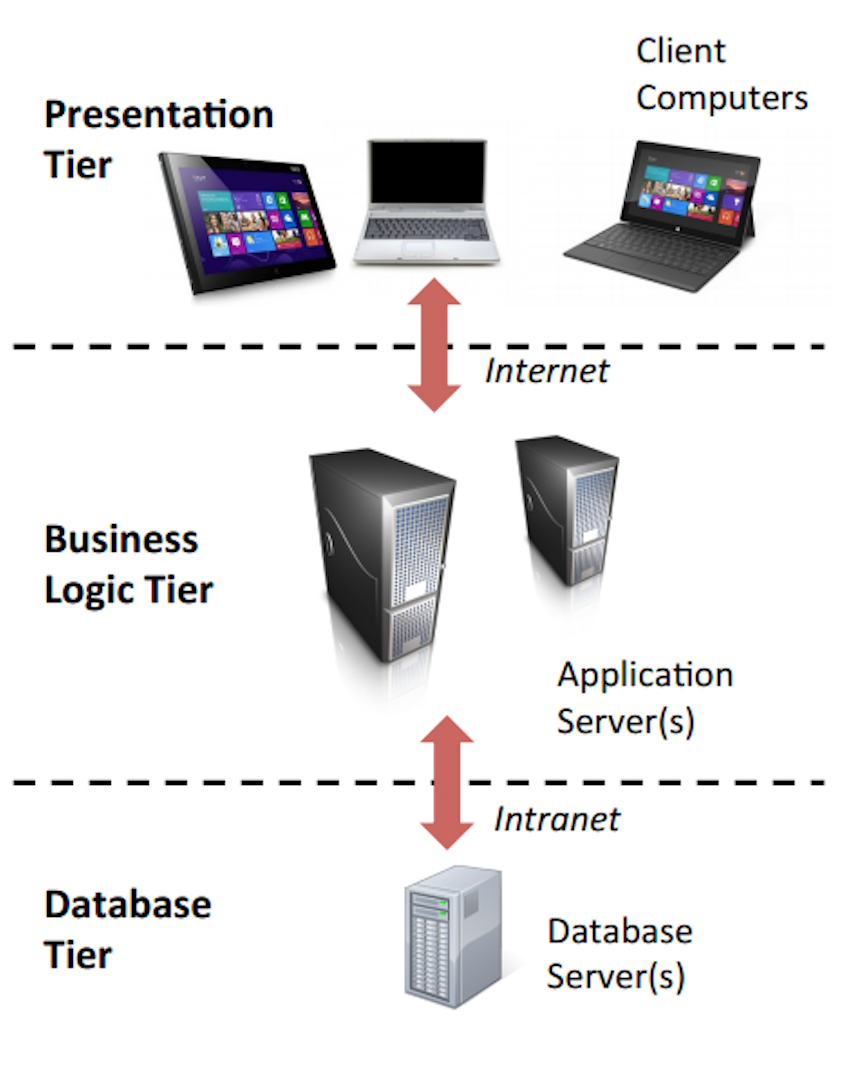
\includegraphics[width=0.5\linewidth]{figs/arkitektur/3tier}
	\caption{ 3-Tier}
	\label{fig:3tier}
\end{figure}

Figur~\ref{fig:3tier} viser tre tiers, som repræsenterer hvert sit ansvarsområde, som ønskes afkoblet. I det følgende vil de tre tiers blive beskrevet.

\begin{figure}
	\centering
	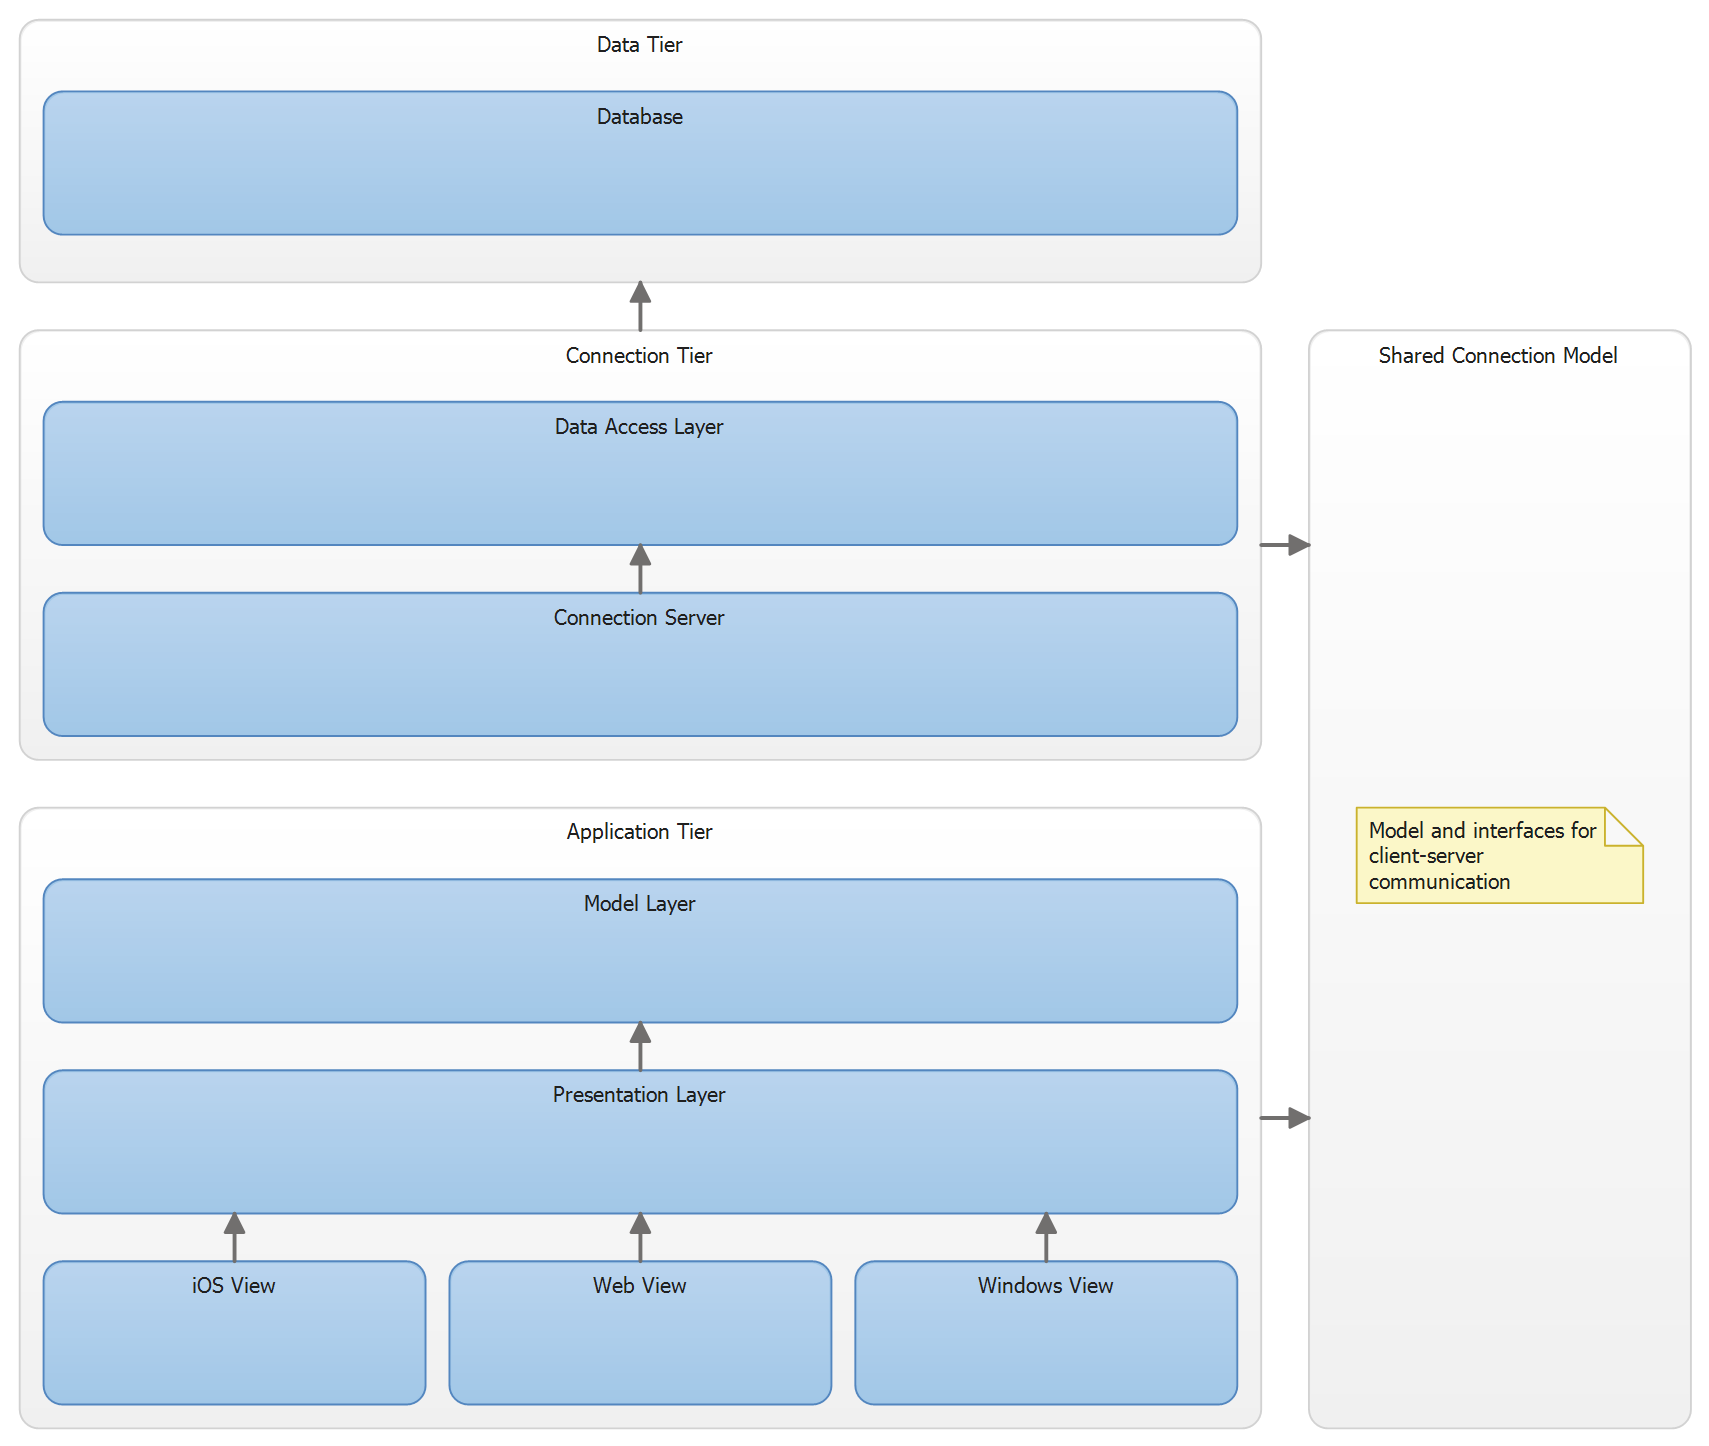
\includegraphics[width=0.9\linewidth]{figs/arkitektur/Smartpool_tiersnlayers}
	\caption{Tiers and layers}
	\label{fig:tiersnlayers}
\end{figure}

\subsection{Presentation Tier}
Det ønskes at afkoble view fra præsentationslogikken og modellen. Til det formål benyttes GUI arkitekturen MVP. Det bruges så viewet er afkoblet og dermed kan udskiftes. Det er gjort med henblik på, at genbruge præsentationslogikken på flere platforme. Arkitekturen understøtter dermed kravene til projektet om som minimum et Windows GUI, med mulighed for udvidelse til iOS og web. Presentation tier kommunikerer med Business Logic tier igennem en Shared Connection Model jf. figur \ref{fig:tiersnlayers}. 

\subsection{Business Logic Tier}
Da det ønskes at adskille systemets business logic fra brugerens applikation, er der oprettet en server som står for dette. Da systemets primære opgave er at gemme og vise data, består dette primært i at lave kald til databasen. Ved at have disse kald i en separat server applikation, sikrer vi at brugerens adgang til databasen, kun går gennem serveren, som dermed kan beskytte de kritiske data.

\subsection{Database Tier}

\section{4+1 Arkitektur Model}
Systemets arkitektur beskrives ved 4+1 modellen. \todo{fodnote eller ref til 4+1}

\todo{Selve modellen skal ikke beskrives her lav en reference til info om 4+1}


\begin{itemize}
	\item \textbf{Logical view} - End-user funktionalitet
	\begin{itemize}
		\item Klassediagrammer, Package diagram, State machine diagram.
	\end{itemize}
	\item \textbf{Process view} - Adfærd og performance
	\begin{itemize}
		\item Activity diagram, Sekvens diagram.
	\end{itemize}
	\item \textbf{Implementation/Development view} - Udviklerperspektivet
	\begin{itemize}
		\item Component diagram.
	\end{itemize}
	\item \textbf{Physical view} - Fysiske bindinger i systemet
	\begin{itemize}
		\item Deployment diagram.
	\end{itemize}
\end{itemize}

\begin{figure}[h]
	\centering
	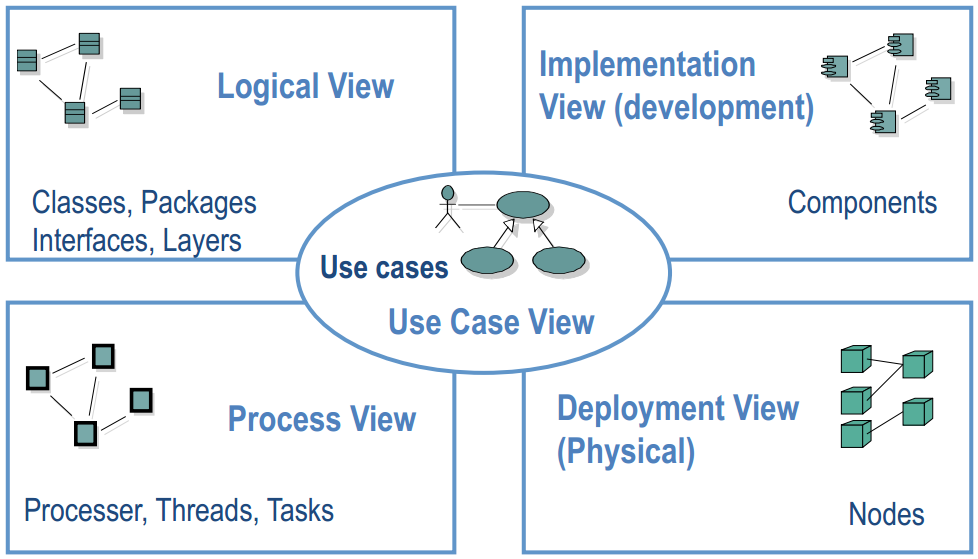
\includegraphics[width=0.9\linewidth]{figs/arkitektur/41model}
	\caption{$4+1$ Arkitektur modellen \cite{flylib}}
	\label{fig:41model}
\end{figure}
\todo{Beskriv i metode eller whatever}

\subsection{Logical view}
Logical view beskriver funktionaliteten for systemets end-user. Logical view repræsenteres ved et Activity diagram. Figur \ref{fig:ActivityDiagram} illustrerer et typisk brugsscenarie for en end-user. 
\begin{figure}
\centering
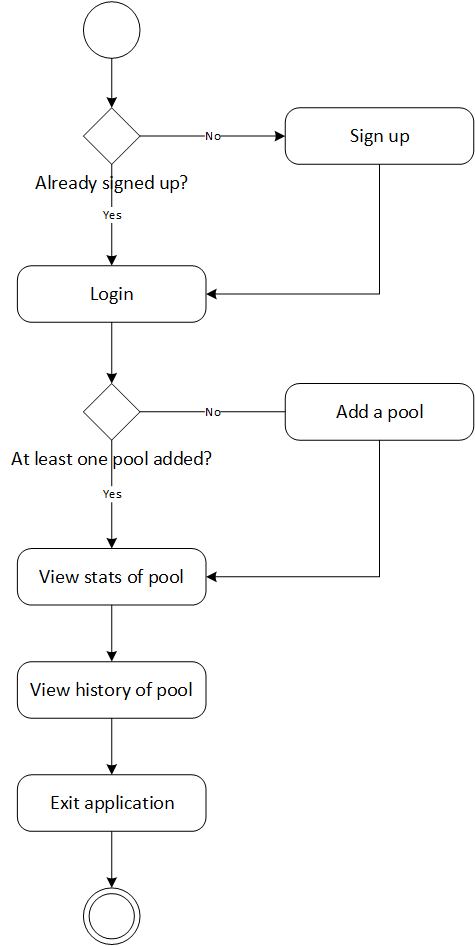
\includegraphics[width=0.55\linewidth]{figs/arkitektur/ActivityDiagram.PNG}
\caption{Activity diagram}
\label{fig:ActivityDiagram}
\end{figure}

\subsection{Process view}
Dette view beskriver systemets concurrency. Systemet håndterer at flere typer platforme kan tilgå serveren og modtage data på samme tid. Dette fremgår af Figur~\ref{fig:processview}
\begin{figure}
\centering
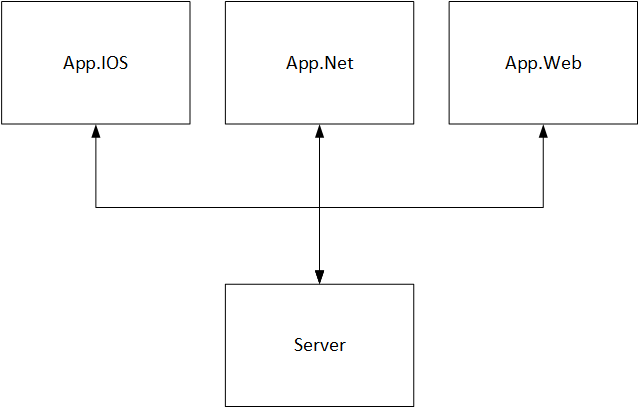
\includegraphics[width=0.7\linewidth]{figs/arkitektur/Processview.png}
\caption{Process view}
\label{fig:processview}

\subsection{Development view}
Dette view illustrerer systemet fra udviklers perspektiv og omhandler software håndtering. Viewet beskrives vha. et komponentdiagram. Viewet er lavet ved at analyserer lag modellen \ref{fig:Smartpool_tiersnlayers} og det Logical view. Alle GUI's bruger Connection komponentens interface. Connection bruger Data Access lagets interface ISmartpoolDB. Data Access laget kommunikerer med databasen vha. Entity Frameworket.

\todo{skal laves om... der mangler web. Omdøb data connection til Connection}
\begin{figure}
\centering
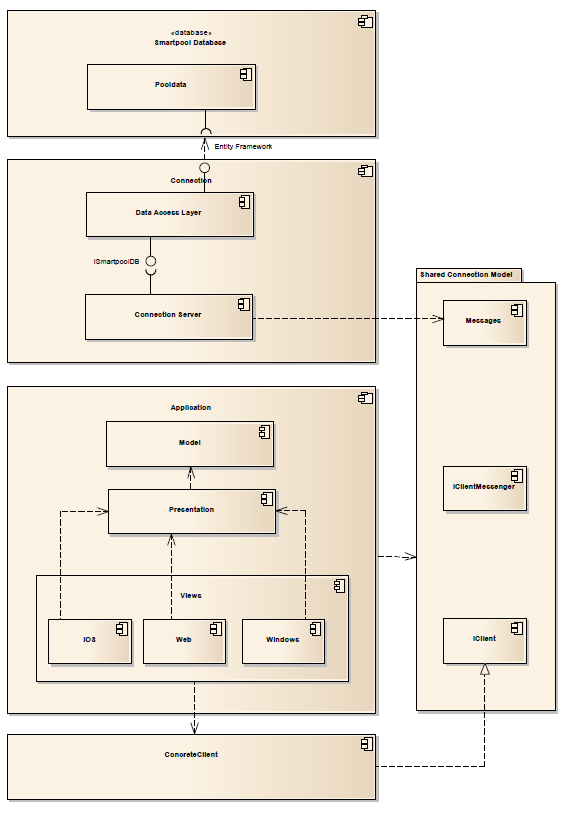
\includegraphics[width=0.7\linewidth]{figs/arkitektur/componentModel}
\caption{Component model for Smartpool systemet}
\label{fig:componentModel}
\end{figure}

\section{Physical view}
Dette view beskriver software komponenternes fysiske placering og den fysiske forbindelse imellem de fysiske placeringer. Det vises ved et Deployment diagram, som udvilkes ved at identificerer, hvor de forskellige komponenter i figur\ref{fig:componentModel}. Diagrammet viser, hvordan de tre fysiske klienter tilgår connection server med TCP/IP. Connection serveren tilgår databsen 
På figur \ref{fig:deploymentView} ses projektets deployment diagram.

\todo{connection skal ud på alle clienter web, iOs, Win // Web server indeholder ASP.NET MVC // SQL skal laves om til TCP/IP}
\begin{figure}
	\centering
	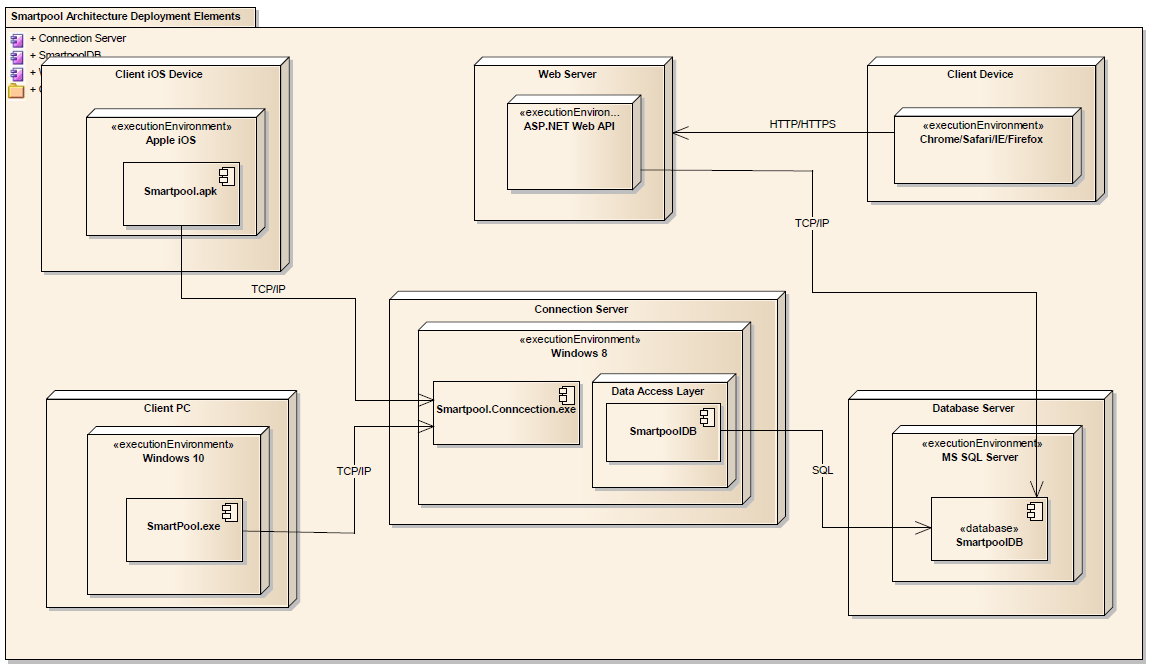
\includegraphics[width=\linewidth]{figs/arkitektur/deploymentView.PNG}
	\caption{Deployment diagram - Physical view}
	\label{fig:deploymentView}
>>>>>>> 4f0387033f0b8e0f2cdcfb0f323be6486c07155f
\end{figure}

\section{Use case view}
I projektet bruges user stories til at beskrive systemets brugsscenarier. Disse User Stories kan ses i afsnittet \todo{reference til US}.

